\documentclass[11pt,a4paper]{article}

% ── Packages ──────────────────────────────────────────────
\usepackage[utf8]{inputenc}
\usepackage[T1]{fontenc}
\usepackage{lmodern}
\usepackage[margin=2.4cm]{geometry}
\usepackage{amsmath,amssymb,amsthm}
\usepackage{mathtools}
\usepackage{physics}
\usepackage{tikz}
\usetikzlibrary{arrows.meta,decorations.markings,positioning,calc,fit,backgrounds}
\usepackage{xcolor}
\usepackage{tcolorbox}
\tcbuselibrary{skins,breakable}
\usepackage{enumitem}
\usepackage{booktabs}
\usepackage{hyperref}
\hypersetup{colorlinks,linkcolor=blue!60!black,citecolor=green!50!black,urlcolor=blue!70!black}
\usepackage{cleveref}

% ── Colours ───────────────────────────────────────────────
\definecolor{ketcol}{RGB}{40,100,180}     % blue  — ket MPS
\definecolor{bracol}{RGB}{180,60,60}      % red   — bra MPS
\definecolor{mpocol}{RGB}{50,140,80}      % green — MPO
\definecolor{envcol}{RGB}{160,120,40}     % gold  — environment
\definecolor{fusecol}{RGB}{100,60,160}    % purple — fusion node
\definecolor{splitcol}{RGB}{200,100,40}   % orange — splitting node
\definecolor{Fcol}{RGB}{180,50,130}       % magenta — F-move
\definecolor{Rcol}{RGB}{0,150,150}        % teal — R-symbol / swap
\definecolor{revcol}{RGB}{200,60,60}      % red — reversal
\definecolor{lightbg}{RGB}{248,248,255}

% ── TikZ styles ──────────────────────────────────────────
\tikzset{
  % directed edge: arrow at midpoint
  directed/.style={
    decoration={markings, mark=at position 0.55 with {\arrow{Stealth[length=5pt,width=3.5pt]}}},
    postaction={decorate}
  },
  % reversed directed edge
  rdirected/.style={
    decoration={markings, mark=at position 0.55 with {\arrowreversed{Stealth[length=5pt,width=3.5pt]}}},
    postaction={decorate}
  },
  % fusion node
  fnode/.style={circle, draw=fusecol, fill=fusecol!15, inner sep=1.5pt, minimum size=6pt, font=\tiny},
  % splitting node
  snode/.style={circle, draw=splitcol, fill=splitcol!15, inner sep=1.5pt, minimum size=6pt, font=\tiny},
  % tensor box
  tbox/.style={rectangle, rounded corners=3pt, draw=#1, fill=#1!8, minimum width=14mm, minimum height=8mm,
               font=\small\bfseries, inner sep=3pt},
  tbox/.default={black},
  % small tensor box
  stbox/.style={rectangle, rounded corners=2pt, draw=#1, fill=#1!8, minimum width=10mm, minimum height=6mm,
               font=\footnotesize\bfseries, inner sep=2pt},
  stbox/.default={black},
  % operation label
  oplabel/.style={font=\footnotesize\sffamily\bfseries, #1},
  oplabel/.default={Fcol},
  % step arrow
  steparrow/.style={-{Stealth[length=6pt]}, thick, #1},
  steparrow/.default={black!60},
  % phantom for alignment
  phantomnode/.style={inner sep=0pt, outer sep=0pt, minimum size=0pt},
}

% ── tcolorbox styles ─────────────────────────────────────
\newtcolorbox{strategybox}[1][]{
  enhanced, breakable,
  colback=blue!3, colframe=ketcol!70!black,
  boxrule=0.6pt, arc=3pt,
  fonttitle=\bfseries\sffamily, title={#1},
  top=4pt, bottom=4pt
}

\newtcolorbox{rulebox}[1][]{
  enhanced,
  colback=yellow!4, colframe=envcol!80!black,
  boxrule=0.5pt, arc=2pt,
  fonttitle=\bfseries\sffamily\small, title={#1},
  top=3pt, bottom=3pt
}

\newtcolorbox{costbox}{
  enhanced,
  colback=green!3, colframe=mpocol!70!black,
  boxrule=0.5pt, arc=2pt,
  top=3pt, bottom=3pt
}

% ── Macros ────────────────────────────────────────────────
\newcommand{\SU}{\mathrm{SU}(2)}
\newcommand{\Fmove}{\mathcal{F}}
\newcommand{\Rsym}{\mathcal{R}}
\newcommand{\CG}{C^{\mathrm{fuse}}}
\newcommand{\CGsplit}{C^{\mathrm{split}}}
\newcommand{\degblock}{P}
\newcommand{\ida}{\mathrm{id}}

\title{\bfseries\sffamily
  $\boldsymbol{SU(2)}$-Symmetric Finite vMPS:\\[4pt]
  Tensor Manipulation Strategy\\[2pt]
  {\large\mdseries Using Simple Fusion Trees Without Monster Trees}}
\author{}
\date{}

% ══════════════════════════════════════════════════════════
\begin{document}
\maketitle
\thispagestyle{empty}

\begin{abstract}
\noindent
We present a self-contained account of how to implement a finite variational
Matrix Product State (vMPS) algorithm with global $\SU$ symmetry, following
the fusion-tree strategy of Schmoll, Singh, Rizzi, and Or\'us~\cite{SSRO2019}.
The central idea is to store every tensor in a fixed \emph{canonical simple
fusion tree} and reduce all structural manipulations to a small set of local
moves: $F$-moves (recoupling), $R$-symbol sibling swaps, and boundary index
reversals.  We spell out, for each tensor operation arising in a two-site
finite-vMPS sweep, the exact sequence of these elementary steps, and
illustrate every stage with diagrammatic figures.
\end{abstract}

\tableofcontents
\newpage

% ══════════════════════════════════════════════════════════
\section{Overview of the Strategy}
\label{sec:overview}

\subsection{The problem}

In a finite vMPS sweep one repeatedly performs four operations:
\begin{enumerate}[label=(\roman*),nosep]
  \item \textbf{MPS canonicalization} — bring the MPS into left- or right-canonical form up to a chosen centre site;
  \item \textbf{Environment update} — contract the left/right environment tensor with the bra, MPO, and ket at the next site;
  \item \textbf{Effective-Hamiltonian application} — apply $H_{\mathrm{eff}} = L \cdot W_i \cdot W_{i+1} \cdot R$ to the two-site tensor $\Theta$ inside a Lanczos iteration;
  \item \textbf{Two-site SVD} — split the optimised $\Theta$ back into two MPS tensors with truncation.
\end{enumerate}

When $\SU$ symmetry is imposed, every tensor carries a \emph{fusion tree} that
encodes how the irrep labels on its legs couple.  Na\"ive contraction of
higher-rank symmetric tensors can produce \emph{monster fusion trees} — trees
that cannot be reduced to simple form by $F$-moves alone.  The strategy of
Ref.~\cite{SSRO2019} avoids this entirely:

\begin{strategybox}[Core Principle]
\begin{enumerate}[nosep]
  \item Choose one \textbf{canonical simple fusion tree} for each tensor type and store all cached tensors in that tree.
  \item Choose \textbf{contraction orders} so that contracted legs always meet at a common parent node.
  \item Use only \textbf{local} $F$-moves, sibling swaps ($R$-symbols), and boundary index reversals before each contraction.
\end{enumerate}
\end{strategybox}

\subsection{Elementary moves}

All structural work is decomposed into three primitives, ordered by preference:

\begin{rulebox}[Hierarchy of Structural Operations]
\begin{enumerate}[nosep,label=\arabic*.]
  \item \textcolor{Fcol}{\bfseries$F$-move} — recouple two adjacent fusion nodes; changes which pair of legs share a parent.
        The degeneracy blocks transform as $\degblock'_y = \sum_x (F^{-1})_{xy}\,\degblock_x$.
  \item \textcolor{Rcol}{\bfseries Sibling swap ($R$-symbol)} — exchange the two children of a single node.
        Costs only a sign: $(-1)^{j_a + j_b - j_c}$ per block.
  \item \textcolor{revcol}{\bfseries Index reversal} — flip the direction of a \emph{boundary} leg using a CUP/CAP insertion.
        For $\SU$, this is a scalar factor $(-1)^{j-m}\sqrt{2j+1}$ per component.
\end{enumerate}
\end{rulebox}

\noindent
No generic long-range permutation is ever needed.  If a reversal would hit an internal leg, first
use $F$-moves to push that leg to the boundary.

% ══════════════════════════════════════════════════════════
\section{Tensors and Their Canonical Fusion Trees}
\label{sec:tensors}

We define the five tensor types used in a finite-vMPS sweep together with their
canonical simple fusion trees.  In every diagram below:
\begin{itemize}[nosep]
  \item Arrows indicate the direction of the index ($\to$ = incoming, $\leftarrow$ = outgoing).
  \item \tikz[baseline=-2pt]{\node[fnode]{};} = fusion node \quad
        \tikz[baseline=-2pt]{\node[snode]{};} = splitting node.
  \item Colours:
        \textcolor{ketcol}{blue = ket MPS},
        \textcolor{bracol}{red = bra MPS},
        \textcolor{mpocol}{green = MPO},
        \textcolor{envcol}{gold = environment}.
\end{itemize}

% ── 2.1 Ket MPS ──────────────────────────────────────────
\subsection{Ket MPS tensor $A(a_l, p, a_r)$}

\begin{center}
\begin{tikzpicture}[scale=1.0]
  % fusion node
  \node[fnode, label={[fusecol,font=\scriptsize]right:fuse}] (f) at (0,0) {};
  % legs
  \draw[directed, ketcol, thick] (-1.8,0) node[left,font=\small]{$a_l$} -- (f);
  \draw[directed, ketcol, thick] (0,1.4) node[above,font=\small]{$p$} -- (f);
  \draw[directed, ketcol, thick] (f) -- (1.8,0) node[right,font=\small]{$a_r$};
  % labels
  \node[below=6pt, font=\footnotesize\itshape, text=black!60] at (0,-0.3)
    {$(a_l, p) \to a_r$};
\end{tikzpicture}
\end{center}

Index 0 ($a_l$): left virtual, \textbf{incoming}.
Index 1 ($p$): physical, \textbf{incoming}.
Index 2 ($a_r$): right virtual, \textbf{outgoing}.

The single fusion node reads: ``fuse the left virtual and physical irreps to
produce the right virtual irrep.''

% ── 2.2 Bra MPS ──────────────────────────────────────────
\subsection{Bra MPS tensor $B(b_l, \bar{p}, b_r) = A^\dagger$}

\begin{center}
\begin{tikzpicture}[scale=1.0]
  \node[snode, label={[splitcol,font=\scriptsize]right:split}] (s) at (0,0) {};
  \draw[directed, bracol, thick] (s) -- (-1.8,0) node[left,font=\small]{$b_l$};
  \draw[directed, bracol, thick] (s) -- (0,-1.4) node[below,font=\small]{$\bar{p}$};
  \draw[directed, bracol, thick] (1.8,0) node[right,font=\small]{$b_r$} -- (s);
  \node[above=6pt, font=\footnotesize\itshape, text=black!60] at (0,0.3)
    {$b_r \to (b_l, \bar{p})$};
\end{tikzpicture}
\end{center}

This is the natural dual of $A$.  Index $b_r$ is \textbf{incoming};
indices $b_l$ and $\bar{p}$ are \textbf{outgoing}.  The splitting node decomposes
the right virtual irrep into the left virtual and conjugate physical irreps.

% ── 2.3 MPO ──────────────────────────────────────────────
\subsection{MPO tensor $W(w_l, \bar{p}, p, w_r)$}

\begin{center}
\begin{tikzpicture}[scale=1.0]
  % two fusion nodes
  \node[fnode] (f1) at (0,0.6) {};
  \node[fnode] (f2) at (0,-0.6) {};
  % legs
  \draw[directed, mpocol, thick] (-1.8,0.6) node[left,font=\small]{$w_l$} -- (f1);
  \draw[directed, mpocol, thick] (0,2.0) node[above,font=\small]{$\bar{p}$} -- (f1);
  \draw[directed, mpocol, thick] (f1) -- (f2) node[midway, right, font=\scriptsize, text=fusecol]{$x$};
  \draw[directed, mpocol, thick] (0,-2.0) node[below,font=\small]{$p$} -- (f2);
  \draw[directed, mpocol, thick] (f2) -- (1.8,-0.6) node[right,font=\small]{$w_r$};
  % labels
  \node[right=18pt, font=\footnotesize\itshape, text=black!60, align=left] at (1.8,0)
    {$(w_l, \bar{p}) \to x$\\$(x,\; p\;) \to w_r$};
\end{tikzpicture}
\end{center}

A two-node chain.  The internal edge $x$ is the single intermediate fusion
channel.  This is already a simple fusion tree.

% ── 2.4 Left environment ─────────────────────────────────
\subsection{Left environment $L(b_l, w_l, a_l)$}

\begin{center}
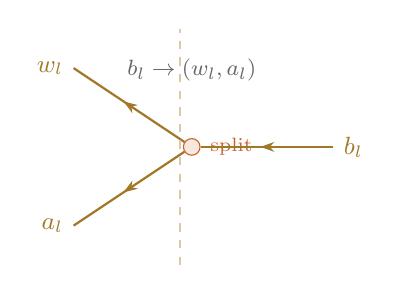
\begin{tikzpicture}[scale=1.0]
  \node[snode, label={[splitcol,font=\scriptsize]right:split}] (s) at (0,0) {};
  \draw[directed, envcol, thick] (s) -- (-1.5, 1.0) node[left,font=\small]{$w_l$};
  \draw[directed, envcol, thick] (s) -- (-1.5,-1.0) node[left,font=\small]{$a_l$};
  \draw[directed, envcol, thick] (1.8,0) node[right,font=\small]{$b_l$} -- (s);
  % boundary
  \draw[envcol!40, dashed, thick] (-0.15,-1.5) -- (-0.15,1.5);
  \node[above=6pt, font=\footnotesize\itshape, text=black!60] at (0,0.5)
    {$b_l \to (w_l, a_l)$};
\end{tikzpicture}
\end{center}

The left environment is a \emph{splitting} tensor: the bra virtual leg $b_l$
(\textbf{incoming}) splits into the MPO virtual $w_l$ and ket virtual $a_l$
(both \textbf{outgoing}).

% ── 2.5 Right environment ────────────────────────────────
\subsection{Right environment $R(a_r, w_r, b_r)$}

\begin{center}
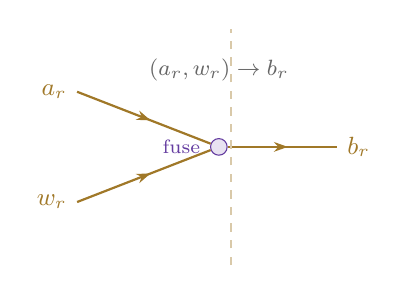
\begin{tikzpicture}[scale=1.0]
  \node[fnode, label={[fusecol,font=\scriptsize]left:fuse}] (f) at (0,0) {};
  \draw[directed, envcol, thick] (-1.8,0.7) node[left,font=\small]{$a_r$} -- (f);
  \draw[directed, envcol, thick] (-1.8,-0.7) node[left,font=\small]{$w_r$} -- (f);
  \draw[directed, envcol, thick] (f) -- (1.5,0) node[right,font=\small]{$b_r$};
  \draw[envcol!40, dashed, thick] (0.15,-1.5) -- (0.15,1.5);
  \node[above=6pt, font=\footnotesize\itshape, text=black!60] at (0,0.5)
    {$(a_r, w_r) \to b_r$};
\end{tikzpicture}
\end{center}

The right environment is a \emph{fusion} tensor: the ket virtual $a_r$ and
MPO virtual $w_r$ (both \textbf{incoming}) fuse to the bra virtual $b_r$
(\textbf{outgoing}).

% ── 2.6 Two-site tensor ──────────────────────────────────
\subsection{Two-site tensor $\Theta(a_l, p_1, p_2, a_r)$}

\begin{center}
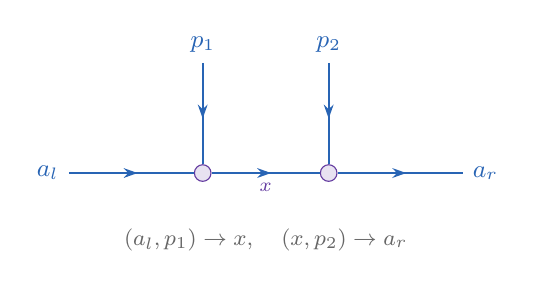
\begin{tikzpicture}[scale=1.0]
  \node[fnode] (f1) at (-0.8,0) {};
  \node[fnode] (f2) at (0.8,0) {};
  \draw[directed, ketcol, thick] (-2.5,0) node[left,font=\small]{$a_l$} -- (f1);
  \draw[directed, ketcol, thick] (-0.8,1.4) node[above,font=\small]{$p_1$} -- (f1);
  \draw[directed, ketcol, thick] (f1) -- (f2) node[midway, below, font=\scriptsize, text=fusecol]{$x$};
  \draw[directed, ketcol, thick] (0.8,1.4) node[above,font=\small]{$p_2$} -- (f2);
  \draw[directed, ketcol, thick] (f2) -- (2.5,0) node[right,font=\small]{$a_r$};
  \node[below=8pt, font=\footnotesize\itshape, text=black!60] at (0,-0.3)
    {$(a_l, p_1) \to x,\quad (x, p_2) \to a_r$};
\end{tikzpicture}
\end{center}

The two-site tensor is simply two ket-MPS fusion nodes chained through the
bond $x$.  Building $\Theta$ from $A_i \cdot A_{i+1}$ by contracting over their
shared bond produces this tree \emph{directly} — no $F$-move, permutation, or
reversal is needed.

% ══════════════════════════════════════════════════════════
\section{MPS Canonicalization}
\label{sec:canon}

\subsection{Left-canonicalization of site $i$}

The ket tensor $A_i$ is already stored in the canonical tree $(a_{i-1}, p_i) \to a_i$.
This is a matrix from the fused incoming leg $\alpha = (a_{i-1}, p_i)$ to the
outgoing leg $a_i$.

\begin{center}
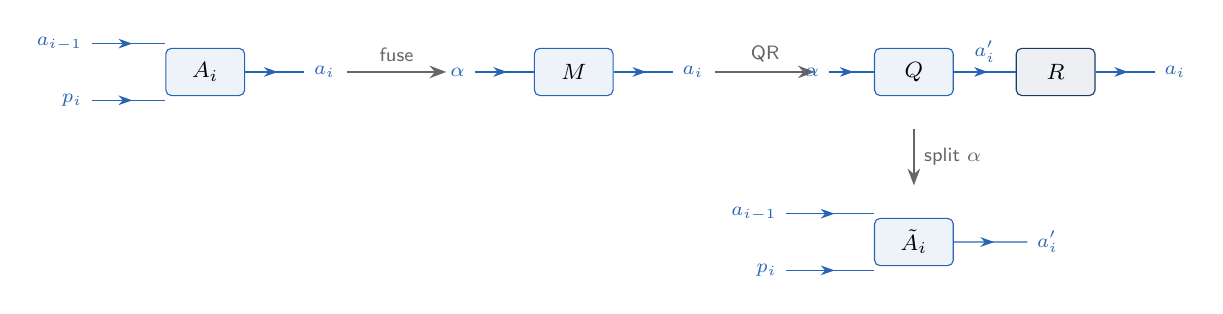
\begin{tikzpicture}[scale=0.9]
  % Step 1: original
  \node[stbox=ketcol] (A) at (0,0) {$A_i$};
  \draw[directed, ketcol] (-1.6,0.4) node[left,font=\scriptsize]{$a_{i-1}$} -- (A.west |- 0,0.4);
  \draw[directed, ketcol] (-1.6,-0.4) node[left,font=\scriptsize]{$p_i$} -- (A.west |- 0,-0.4);
  \draw[directed, ketcol] (A.east) -- (1.4,0) node[right,font=\scriptsize]{$a_i$};

  % arrow
  \draw[steparrow] (2.0,0) -- node[above,font=\scriptsize\sffamily]{fuse} (3.4,0);

  % Step 2: fused
  \node[stbox=ketcol] (M) at (5.2,0) {$M$};
  \draw[directed, ketcol] (3.8,0) node[left,font=\scriptsize]{$\alpha$} -- (M.west);
  \draw[directed, ketcol] (M.east) -- (6.6,0) node[right,font=\scriptsize]{$a_i$};

  % arrow
  \draw[steparrow] (7.2,0) -- node[above,font=\scriptsize\sffamily]{QR} (8.6,0);

  % Step 3: QR
  \node[stbox=ketcol] (Q) at (10.0,0) {$Q$};
  \node[stbox=ketcol!60!black] (R) at (12.0,0) {$R$};
  \draw[directed, ketcol] (8.8,0) node[left,font=\scriptsize]{$\alpha$} -- (Q.west);
  \draw[directed, ketcol] (Q.east) -- (R.west) node[midway,above,font=\scriptsize]{$a'_i$};
  \draw[directed, ketcol] (R.east) -- (13.4,0) node[right,font=\scriptsize]{$a_i$};

  % split arrow
  \draw[steparrow] (10.0,-0.8) -- node[right,font=\scriptsize\sffamily]{split $\alpha$} (10.0,-1.6);

  % Step 4: result
  \node[stbox=ketcol] (Qf) at (10.0,-2.4) {$\tilde A_i$};
  \draw[directed, ketcol] (8.2,-2.0) node[left,font=\scriptsize]{$a_{i-1}$} -- (Qf.west |- 0,-2.0);
  \draw[directed, ketcol] (8.2,-2.8) node[left,font=\scriptsize]{$p_i$} -- (Qf.west |- 0,-2.8);
  \draw[directed, ketcol] (Qf.east) -- (11.6,-2.4) node[right,font=\scriptsize]{$a'_i$};
\end{tikzpicture}
\end{center}

\begin{costbox}
\textbf{Structural cost:} No $F$-move. No permutation. No reversal. \\
The fusion tree is already in the correct form for matrixisation.
\end{costbox}

\subsection{Right-canonicalization of site $i$}

The stored tree $(a_{i-1}, p_i) \to a_i$ is \emph{not} directly a matrix with
$a_{i-1}$ as the outgoing (column) index.  We need one temporary reversal of
the physical leg.

\begin{center}
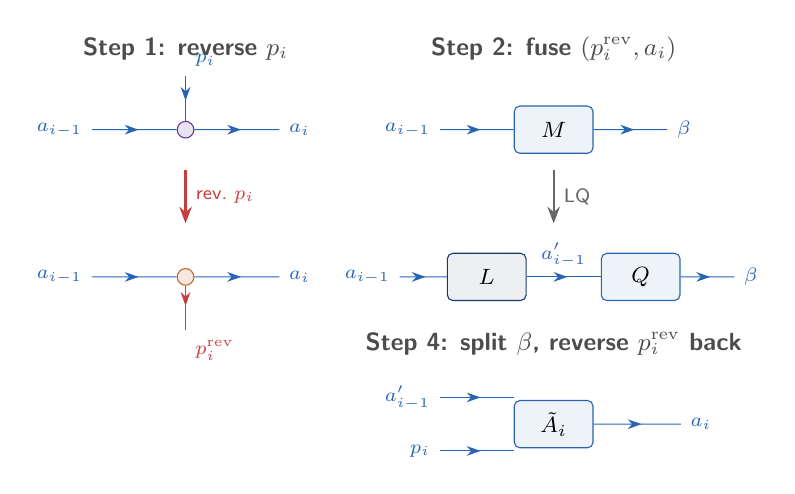
\begin{tikzpicture}[scale=0.85]
  % Step 1
  \node[font=\small\bfseries\sffamily, text=black!70] at (0,1.8) {Step 1: reverse $p_i$};
  \node[fnode] (f1) at (0,0.6) {};
  \draw[directed, ketcol] (-1.4,0.6) node[left,font=\scriptsize]{$a_{i-1}$} -- (f1);
  \draw[directed, ketcol] (0,1.4) node[above right,font=\scriptsize]{$p_i$} -- (f1);
  \draw[directed, ketcol] (f1) -- (1.4,0.6) node[right,font=\scriptsize]{$a_i$};

  \draw[steparrow=revcol] (0,0) -- node[right,font=\scriptsize\sffamily,text=revcol]{rev.\ $p_i$} (0,-0.8);

  % After reversal: splitting node
  \node[snode] (s1) at (0,-1.6) {};
  \draw[directed, ketcol] (-1.4,-1.6) node[left,font=\scriptsize]{$a_{i-1}$} -- (s1);
  \draw[rdirected, revcol] (0,-2.4) node[below right,font=\scriptsize,text=revcol]{$p_i^{\mathrm{rev}}$} -- (s1);
  \draw[directed, ketcol] (s1) -- (1.4,-1.6) node[right,font=\scriptsize]{$a_i$};

  % Step 2
  \node[font=\small\bfseries\sffamily, text=black!70] at (5.5,1.8) {Step 2: fuse $(p_i^{\mathrm{rev}}, a_i)$};
  \node[stbox=ketcol] (M2) at (5.5,0.6) {$M$};
  \draw[directed, ketcol] (3.8,0.6) node[left,font=\scriptsize]{$a_{i-1}$} -- (M2.west);
  \draw[directed, ketcol] (M2.east) -- (7.2,0.6) node[right,font=\scriptsize]{$\beta$};

  % Step 3
  \draw[steparrow] (5.5,0) -- node[right,font=\scriptsize\sffamily]{LQ} (5.5,-0.8);
  \node[stbox=ketcol!60!black] (L2) at (4.5,-1.6) {$L$};
  \node[stbox=ketcol] (Q2) at (6.8,-1.6) {$Q$};
  \draw[directed, ketcol] (3.2,-1.6) node[left,font=\scriptsize]{$a_{i-1}$} -- (L2.west);
  \draw[directed, ketcol] (L2.east) -- (Q2.west) node[midway,above,font=\scriptsize]{$a'_{i-1}$};
  \draw[directed, ketcol] (Q2.east) -- (8.2,-1.6) node[right,font=\scriptsize]{$\beta$};

  % Step 4
  \node[font=\small\bfseries\sffamily, text=black!70] at (5.5,-2.6) {Step 4: split $\beta$, reverse $p_i^{\mathrm{rev}}$ back};
  \node[stbox=ketcol] (Af) at (5.5,-3.8) {$\tilde A_i$};
  \draw[directed, ketcol] (3.8,-3.4) node[left,font=\scriptsize]{$a'_{i-1}$} -- (Af.west |- 0,-3.4);
  \draw[directed, ketcol] (3.8,-4.2) node[left,font=\scriptsize]{$p_i$} -- (Af.west |- 0,-4.2);
  \draw[directed, ketcol] (Af.east) -- (7.4,-3.8) node[right,font=\scriptsize]{$a_i$};
\end{tikzpicture}
\end{center}

\begin{costbox}
\textbf{Structural cost:} One temporary physical-leg reversal (boundary leg,
sector-wise scalar). No $F$-move. No permutation.
\end{costbox}


% ══════════════════════════════════════════════════════════
\section{Left Environment Update}
\label{sec:lenv}

We update
\[
  L_n(b_l, w_l, a_l) + B_n + W_n + A_n \;\longrightarrow\; L_{n+1}(b_r, w_r, a_r).
\]

The contraction order is $((L_n \cdot B_n) \xrightarrow{F} \cdot\, W_n \xrightarrow{F} \cdot\, A_n)$,
chosen so that every intermediate has a simple fusion tree.

\bigskip

% ── MASTER FIGURE: Left environment update ────────────────
\begin{center}
\begin{tikzpicture}[scale=0.78, every node/.style={scale=0.78}]

  % ┌────────────────────────────────────────────┐
  % │  STEP 1: Contract L_n with B_n over b_l   │
  % └────────────────────────────────────────────┘
  \node[font=\normalsize\bfseries\sffamily, text=black!80] at (-5.5,5.5) {Step 1};
  \node[font=\small\itshape, text=black!60] at (-5.5,5.0) {Contract $L_n \cdot B_n$ over $b_l$};

  % L_n
  \node[snode] (Ls) at (-8,3) {};
  \draw[directed, envcol, thick] (-6.5,3) node[right,font=\small]{$b_l$} -- (Ls);
  \draw[directed, envcol, thick] (Ls) -- (-9.5,4) node[left,font=\small]{$w_l$};
  \draw[directed, envcol, thick] (Ls) -- (-9.5,2) node[left,font=\small]{$a_l$};
  \node[font=\scriptsize, envcol] at (-7.6,3.6) {$L_n$};

  % B_n
  \node[snode] (Bs) at (-4,3) {};
  \draw[directed, bracol, thick] (-5.5,3) node[left,font=\small]{$b_l$} -- (Bs) node[midway,above,font=\tiny,text=black!50]{contract};
  \draw[directed, bracol, thick] (Bs) -- (-4,1.5) node[below,font=\small]{$\bar{p}$};
  \draw[directed, bracol, thick] (Bs) -- (-2.5,3) node[right,font=\small]{$b_r$};
  \node[font=\scriptsize, bracol] at (-3.6,3.6) {$B_n$};

  % Result
  \draw[steparrow, thick] (-1.5,3) -- (-0.2,3);

  % Raw tree after contraction
  \node[font=\small\itshape, text=black!60] at (3,5.0) {Raw tree};
  % b_r at top
  \node[snode] (r1) at (2,3.8) {};
  \node[snode] (r2) at (2,2.2) {};
  \draw[directed, black, thick] (3.5,3.8) node[right,font=\small]{$b_r$} -- (r1);
  \draw[directed, black, thick] (r1) -- (0.8,4.6) node[left,font=\small]{$\bar{p}$};
  \draw[directed, black, thick] (r1) -- (r2);
  \draw[directed, black, thick] (r2) -- (0.8,2.8) node[left,font=\small]{$w_l$};
  \draw[directed, black, thick] (r2) -- (0.8,1.6) node[left,font=\small]{$a_l$};
  \node[font=\scriptsize, fusecol, right] at (2.15,3.0) {$x$};

  % ┌────────────────────────────────────────────┐
  % │  STEP 2: F-move                            │
  % └────────────────────────────────────────────┘
  \draw[steparrow=Fcol, very thick] (4.5,3) -- node[above,font=\small\bfseries,text=Fcol]{$\Fmove$} (6.5,3);

  \node[font=\normalsize\bfseries\sffamily, text=Fcol] at (5.5,5.5) {Step 2};
  \node[font=\small\itshape, text=black!60] at (5.5,5.0) {$F$-move: make $(w_l, \bar{p})$ siblings};

  % After F-move
  \node[snode] (f1) at (8.5,3.8) {};
  \node[fnode] (f2) at (8.5,2.2) {};
  \draw[directed, black, thick] (10,3.8) node[right,font=\small]{$b_r$} -- (f1);
  \draw[directed, black, thick] (f1) -- (7.3,4.6) node[left,font=\small]{$a_l$};
  \draw[directed, black, thick] (f1) -- (f2);
  \draw[directed, black, thick] (7.3,2.8) node[left,font=\small]{$w_l$} -- (f2);
  \draw[directed, black, thick] (7.3,1.6) node[left,font=\small]{$\bar{p}$} -- (f2);
  \node[font=\scriptsize, fusecol, right] at (8.65,3.0) {$y$};

  % Formula
  \node[font=\footnotesize, text=Fcol, align=center] at (8.5,0.5)
    {$\degblock_y = \displaystyle\sum_x (F^{-1})_{xy}\,\degblock_x$};

  % ┌────────────────────────────────────────────┐
  % │  STEP 3: optional sibling swap             │
  % └────────────────────────────────────────────┘
  \node[font=\normalsize\bfseries\sffamily, text=Rcol] at (1.5,-1.5) {Step 3};
  \node[font=\small\itshape, text=black!60] at (1.5,-2.0) {Sibling swap if needed};

  \node[font=\footnotesize, text=Rcol, align=center] at (1.5,-3.0)
    {If lower node has $(\bar{p}, w_l)$\\
     swap $\to$ phase $(-1)^{j_{w_l}+j_{\bar{p}}-j_y}$};

  % ┌────────────────────────────────────────────┐
  % │  STEP 4: Contract with W_n                 │
  % └────────────────────────────────────────────┘
  \node[font=\normalsize\bfseries\sffamily, text=black!80] at (6,-1.5) {Step 4};
  \node[font=\small\itshape, text=black!60] at (6,-2.0) {Contract with $W_n$ over $(w_l, \bar{p})$};

  \node[snode] (w1) at (6,-3.5) {};
  \node[fnode] (w2) at (6,-5.1) {};
  \draw[directed, black, thick] (7.5,-3.5) node[right,font=\small]{$b_r$} -- (w1);
  \draw[directed, black, thick] (w1) -- (4.8,-2.7) node[left,font=\small]{$a_l$};
  \draw[directed, black, thick] (w1) -- (w2);
  \draw[directed, black, thick] (4.8,-4.5) node[left,font=\small]{$p$} -- (w2);
  \draw[directed, black, thick] (4.8,-5.7) node[left,font=\small]{$w_r$} -- (w2);
  \node[font=\scriptsize, fusecol, right] at (6.15,-4.3) {$z$};

  % ┌────────────────────────────────────────────┐
  % │  STEP 5: Second F-move                     │
  % └────────────────────────────────────────────┘
  \draw[steparrow=Fcol, very thick] (8.5,-4.3) -- node[above,font=\small\bfseries,text=Fcol]{$\Fmove$} (10.5,-4.3);

  \node[font=\normalsize\bfseries\sffamily, text=Fcol] at (9.5,-1.5) {Step 5};
  \node[font=\small\itshape, text=black!60] at (9.5,-2.0) {$F$-move: make $(a_l, p)$ siblings};

  \node[snode] (g1) at (12,-3.5) {};
  \node[fnode] (g2) at (12,-5.1) {};
  \draw[directed, black, thick] (13.5,-3.5) node[right,font=\small]{$b_r$} -- (g1);
  \draw[directed, black, thick] (g1) -- (10.8,-2.7) node[left,font=\small]{$w_r$};
  \draw[directed, black, thick] (g1) -- (g2);
  \draw[directed, black, thick] (10.8,-4.5) node[left,font=\small]{$a_l$} -- (g2);
  \draw[directed, black, thick] (10.8,-5.7) node[left,font=\small]{$p$} -- (g2);
  \node[font=\scriptsize, fusecol, right] at (12.15,-4.3) {$u$};

  % ┌────────────────────────────────────────────┐
  % │  STEP 6+7: swap + contract with A_n        │
  % └────────────────────────────────────────────┘
  \node[font=\normalsize\bfseries\sffamily, text=Rcol] at (12,-6.5) {Step 6};
  \node[font=\small\itshape, text=black!60] at (12,-7.0) {Optional swap, then};

  \node[font=\normalsize\bfseries\sffamily, text=black!80] at (12,-7.8) {Step 7};
  \node[font=\small\itshape, text=black!60] at (12,-8.3) {Contract with $A_n$ over $(a_l, p)$};

  % Final result
  \draw[steparrow, thick] (12,-8.8) -- (12,-9.5);
  \node[snode] (fin) at (12,-10.5) {};
  \draw[directed, envcol, thick] (13.5,-10.5) node[right,font=\small\bfseries]{$b_r$} -- (fin);
  \draw[directed, envcol, thick] (fin) -- (10.5,-9.7) node[left,font=\small\bfseries]{$w_r$};
  \draw[directed, envcol, thick] (fin) -- (10.5,-11.3) node[left,font=\small\bfseries]{$a_r$};
  \node[font=\small\bfseries, envcol] at (13.5,-11.0) {$= L_{n+1}$};

\end{tikzpicture}
\end{center}

\begin{costbox}
\textbf{Structural cost per left-environment update:}
\begin{itemize}[nosep]
  \item 2 fixed $F$-moves
  \item At most 2 sibling swaps ($R$-phase)
  \item No hot-loop index reversal
  \item No yoga/monster tree
\end{itemize}
\end{costbox}

% ══════════════════════════════════════════════════════════
\section{Right Environment Update}
\label{sec:renv}

The right update is the mirror of the left:
\[
  A_n + W_n + B_n + R_{n+1}(a_r, w_r, b_r) \;\longrightarrow\; R_n(a_l, w_l, b_l).
\]
with contraction order $((A_n \cdot R_{n+1}) \xrightarrow{F} \cdot\, W_n \xrightarrow{F} \cdot\, B_n)$.

\begin{center}
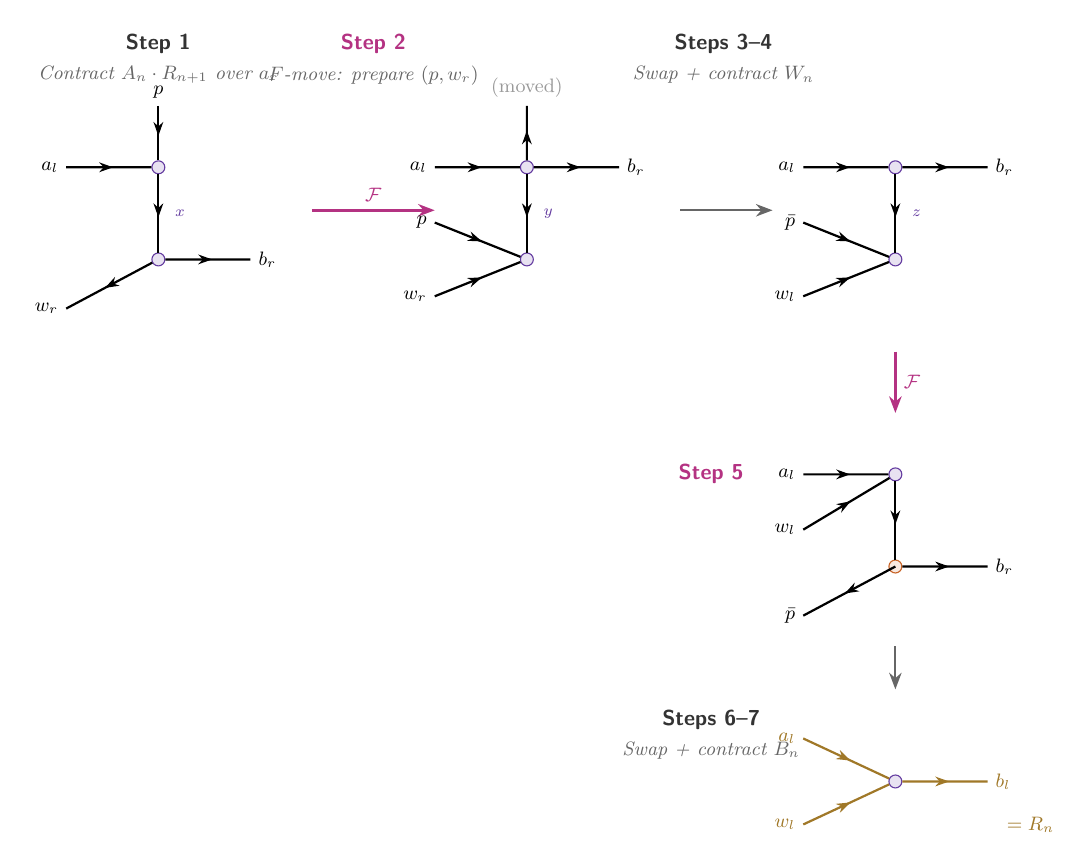
\begin{tikzpicture}[scale=0.78, every node/.style={scale=0.78}]

  % ── STEP 1: Contract A_n · R_{n+1} over a_r ──
  \node[font=\normalsize\bfseries\sffamily, text=black!80] at (0,4.5) {Step 1};
  \node[font=\small\itshape, text=black!60] at (0,4.0) {Contract $A_n \cdot R_{n+1}$ over $a_r$};

  % Raw tree
  \node[fnode] (q1) at (0,2.5) {};
  \node[fnode] (q2) at (0,1.0) {};
  \draw[directed, black, thick] (-1.5,2.5) node[left,font=\small]{$a_l$} -- (q1);
  \draw[directed, black, thick] (q1) -- (q2);
  \draw[directed, black, thick] (0,3.5) node[above,font=\small]{$p$} -- (q1);
  \draw[directed, black, thick] (q2) -- (-1.5,0.2) node[left,font=\small]{$w_r$};
  \draw[directed, black, thick] (q2) -- (1.5,1.0) node[right,font=\small]{$b_r$};
  \node[font=\scriptsize, fusecol, right] at (0.15,1.75) {$x$};

  % ── STEP 2: F-move ──
  \draw[steparrow=Fcol, very thick] (2.5,1.8) -- node[above,font=\small\bfseries,text=Fcol]{$\Fmove$} (4.5,1.8);

  \node[font=\normalsize\bfseries\sffamily, text=Fcol] at (3.5,4.5) {Step 2};
  \node[font=\small\itshape, text=black!60] at (3.5,4.0) {$F$-move: prepare $(p, w_r)$};

  \node[fnode] (h1) at (6,2.5) {};
  \node[fnode] (h2) at (6,1.0) {};
  \draw[directed, black, thick] (4.5,2.5) node[left,font=\small]{$a_l$} -- (h1);
  \draw[directed, black, thick] (h1) -- (h2);
  \draw[directed, black, thick] (h1) -- (6,3.5) node[above,font=\small,text=black!40]{(moved)};
  \draw[directed, black, thick] (4.5,1.6) node[left,font=\small]{$p$} -- (h2);
  \draw[directed, black, thick] (4.5,0.4) node[left,font=\small]{$w_r$} -- (h2);
  \draw[directed, black, thick] (h1) -- (7.5,2.5) node[right,font=\small]{$b_r$};
  \node[font=\scriptsize, fusecol, right] at (6.15,1.75) {$y$};

  % Step 3 (swap) + Step 4 (contract W)
  \draw[steparrow, thick] (8.5,1.8) -- (10,1.8);
  \node[font=\normalsize\bfseries\sffamily, text=black!80] at (9.2,4.5) {Steps 3--4};
  \node[font=\small\itshape, text=black!60] at (9.2,4.0) {Swap + contract $W_n$};

  % After W contraction
  \node[fnode] (k1) at (12,2.5) {};
  \node[fnode] (k2) at (12,1.0) {};
  \draw[directed, black, thick] (10.5,2.5) node[left,font=\small]{$a_l$} -- (k1);
  \draw[directed, black, thick] (k1) -- (k2);
  \draw[directed, black, thick] (10.5,1.6) node[left,font=\small]{$\bar{p}$} -- (k2);
  \draw[directed, black, thick] (10.5,0.4) node[left,font=\small]{$w_l$} -- (k2);
  \draw[directed, black, thick] (k1) -- (13.5,2.5) node[right,font=\small]{$b_r$};
  \node[font=\scriptsize, fusecol, right] at (12.15,1.75) {$z$};

  % ── STEP 5: Second F-move ──
  \draw[steparrow=Fcol, very thick] (12,-0.5) -- node[right,font=\small\bfseries,text=Fcol]{$\Fmove$} (12,-1.5);

  % After second F
  \node[fnode] (m1) at (12,-2.5) {};
  \node[snode] (m2) at (12,-4.0) {};
  \draw[directed, black, thick] (12,-4.0) -- (10.5,-4.8) node[left,font=\small]{$\bar{p}$};
  \draw[directed, black, thick] (10.5,-2.5) node[left,font=\small]{$a_l$} -- (m1);
  \draw[directed, black, thick] (10.5,-3.4) node[left,font=\small]{$w_l$} -- (m1);
  \draw[directed, black, thick] (m1) -- (m2);
  \draw[directed, black, thick] (m2) -- (13.5,-4.0) node[right,font=\small]{$b_r$};

  \node[font=\normalsize\bfseries\sffamily, text=Fcol] at (9,-2.5) {Step 5};

  % ── STEP 6+7: swap + contract B ──
  \draw[steparrow, thick] (12,-5.3) -- (12,-6.0);
  \node[font=\normalsize\bfseries\sffamily, text=black!80] at (9,-6.5) {Steps 6--7};
  \node[font=\small\itshape, text=black!60] at (9,-7.0) {Swap + contract $B_n$};

  % Final
  \node[fnode] (fin) at (12,-7.5) {};
  \draw[directed, envcol, thick] (10.5,-6.8) node[left,font=\small\bfseries]{$a_l$} -- (fin);
  \draw[directed, envcol, thick] (10.5,-8.2) node[left,font=\small\bfseries]{$w_l$} -- (fin);
  \draw[directed, envcol, thick] (fin) -- (13.5,-7.5) node[right,font=\small\bfseries]{$b_l$};
  \node[font=\small\bfseries, envcol] at (14.2,-8.2) {$= R_n$};

\end{tikzpicture}
\end{center}

\begin{costbox}
Same structural cost as the left update:
2 $F$-moves, at most 2 $R$-swaps, no reversal, no monster tree.
\end{costbox}


% ══════════════════════════════════════════════════════════
\section{Two-Site Tensor Construction}
\label{sec:twosite}

Contract neighbouring MPS tensors $A_i(a_l, p_1, m)$ and $A_{i+1}(m, p_2, a_r)$
over the shared bond $m$:

\begin{center}
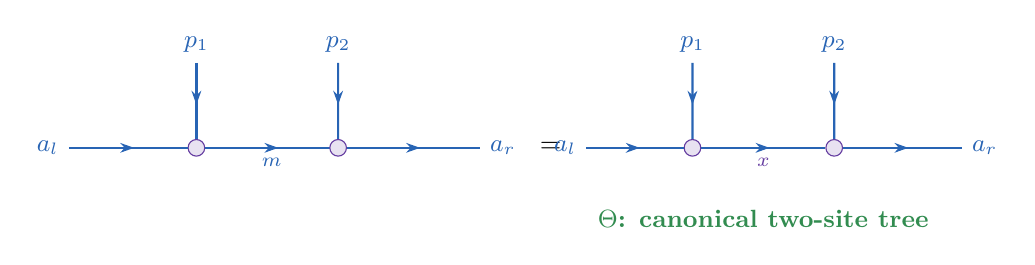
\begin{tikzpicture}[scale=0.9]
  % A_i
  \node[fnode] (f1) at (0,0) {};
  \draw[directed, ketcol, thick] (-1.8,0) node[left,font=\small]{$a_l$} -- (f1);
  \draw[directed, ketcol, thick] (0,1.2) node[above,font=\small]{$p_1$} -- (f1);
  \draw[directed, ketcol, thick] (f1) -- (2,0) node[midway,below,font=\scriptsize]{$m$};

  % A_{i+1}
  \node[fnode] (f2) at (2,0) {};
  \draw[directed, ketcol, thick] (2,1.2) node[above,font=\small]{$p_2$} -- (f2);
  \draw[directed, ketcol, thick] (f2) -- (4,0) node[right,font=\small]{$a_r$};

  % = sign
  \node at (5,0) {$=$};

  % Theta
  \node[fnode] (g1) at (7,0) {};
  \node[fnode] (g2) at (9,0) {};
  \draw[directed, ketcol, thick] (5.5,0) node[left,font=\small]{$a_l$} -- (g1);
  \draw[directed, ketcol, thick] (7,1.2) node[above,font=\small]{$p_1$} -- (g1);
  \draw[directed, ketcol, thick] (g1) -- (g2) node[midway,below,font=\scriptsize,text=fusecol]{$x$};
  \draw[directed, ketcol, thick] (9,1.2) node[above,font=\small]{$p_2$} -- (g2);
  \draw[directed, ketcol, thick] (g2) -- (10.8,0) node[right,font=\small]{$a_r$};

  \node[below=14pt, font=\small\bfseries, text=mpocol] at (8,-0.2) {$\Theta$: canonical two-site tree};
\end{tikzpicture}
\end{center}

\begin{costbox}
\textbf{Structural cost:} None.
The contraction directly produces the canonical two-site tree.
\end{costbox}


% ══════════════════════════════════════════════════════════
\section{Effective-Hamiltonian Application (Lanczos Matvec)}
\label{sec:heff}

This is the most structurally delicate kernel.  The effective Hamiltonian
$H_{\mathrm{eff}} = L_i \cdot W_i \cdot W_{i+1} \cdot R_{i+1}$
is \emph{never built explicitly}.  Instead, we apply it to $\Theta$ as a
sequence of prepared contractions:

\begin{center}
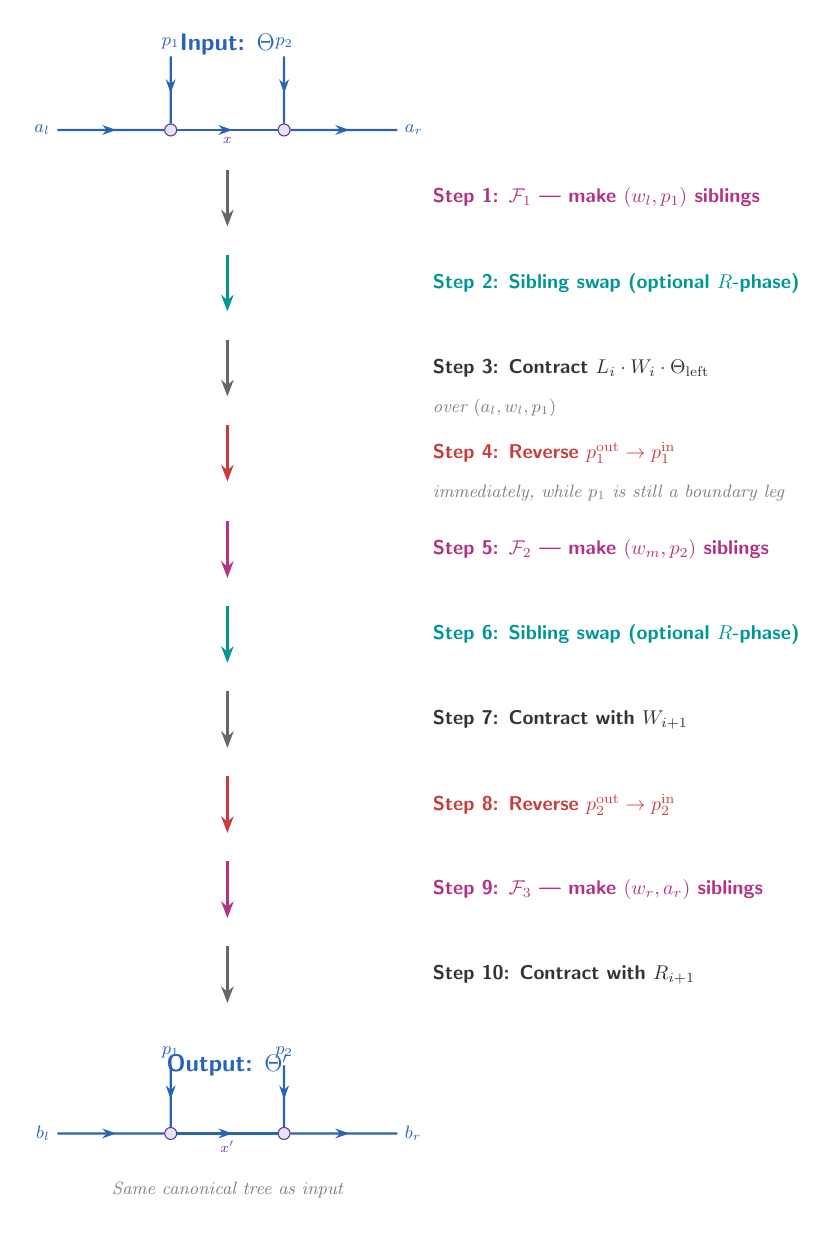
\begin{tikzpicture}[scale=0.72, every node/.style={scale=0.72}]

  % ═══════ INPUT ═══════
  \node[font=\large\bfseries\sffamily, text=ketcol] at (0,8) {Input: $\Theta$};
  \node[fnode] (t1) at (-1,6.5) {};
  \node[fnode] (t2) at (1,6.5) {};
  \draw[directed, ketcol, thick] (-3,6.5) node[left,font=\small]{$a_l$} -- (t1);
  \draw[directed, ketcol, thick] (-1,7.8) node[above,font=\small]{$p_1$} -- (t1);
  \draw[directed, ketcol, thick] (t1) -- (t2) node[midway,below,font=\scriptsize,text=fusecol]{$x$};
  \draw[directed, ketcol, thick] (1,7.8) node[above,font=\small]{$p_2$} -- (t2);
  \draw[directed, ketcol, thick] (t2) -- (3,6.5) node[right,font=\small]{$a_r$};

  % ═══════ LEFT BLOCK ═══════
  % Step 1: F-move to prepare (w_l, p1) as siblings in the combined L+Theta_left
  \draw[steparrow, thick] (0,5.8) -- (0,4.8);
  \node[font=\normalsize\bfseries\sffamily, text=Fcol, anchor=west] at (3.5,5.3)
    {Step 1: $\Fmove_1$ — make $(w_l, p_1)$ siblings};

  % Step 2: swap
  \draw[steparrow=Rcol, thick] (0,4.3) -- (0,3.3);
  \node[font=\normalsize\bfseries\sffamily, text=Rcol, anchor=west] at (3.5,3.8)
    {Step 2: Sibling swap (optional $R$-phase)};

  % Step 3: contract L_i, W_i, left half of Theta
  \draw[steparrow, thick] (0,2.8) -- (0,1.8);
  \node[font=\normalsize\bfseries\sffamily, text=black!80, anchor=west] at (3.5,2.3)
    {Step 3: Contract $L_i \cdot W_i \cdot \Theta_{\mathrm{left}}$};
  \node[font=\small\itshape, text=black!50, anchor=west] at (3.5,1.6)
    {over $(a_l, w_l, p_1)$};

  % Step 4: reverse p1_out -> p1_in
  \draw[steparrow=revcol, thick] (0,1.3) -- (0,0.3);
  \node[font=\normalsize\bfseries\sffamily, text=revcol, anchor=west] at (3.5,0.8)
    {Step 4: Reverse $p_1^{\mathrm{out}} \to p_1^{\mathrm{in}}$};
  \node[font=\small\itshape, text=black!50, anchor=west] at (3.5,0.1)
    {immediately, while $p_1$ is still a boundary leg};

  % ═══════ RIGHT BLOCK ═══════
  % Step 5: F-move
  \draw[steparrow=Fcol, thick] (0,-0.4) -- (0,-1.4);
  \node[font=\normalsize\bfseries\sffamily, text=Fcol, anchor=west] at (3.5,-0.9)
    {Step 5: $\Fmove_2$ — make $(w_m, p_2)$ siblings};

  % Step 6: swap
  \draw[steparrow=Rcol, thick] (0,-1.9) -- (0,-2.9);
  \node[font=\normalsize\bfseries\sffamily, text=Rcol, anchor=west] at (3.5,-2.4)
    {Step 6: Sibling swap (optional $R$-phase)};

  % Step 7: contract W_{i+1}
  \draw[steparrow, thick] (0,-3.4) -- (0,-4.4);
  \node[font=\normalsize\bfseries\sffamily, text=black!80, anchor=west] at (3.5,-3.9)
    {Step 7: Contract with $W_{i+1}$};

  % Step 8: reverse p2_out -> p2_in
  \draw[steparrow=revcol, thick] (0,-4.9) -- (0,-5.9);
  \node[font=\normalsize\bfseries\sffamily, text=revcol, anchor=west] at (3.5,-5.4)
    {Step 8: Reverse $p_2^{\mathrm{out}} \to p_2^{\mathrm{in}}$};

  % ═══════ RIGHT ENV ═══════
  % Step 9: F-move
  \draw[steparrow=Fcol, thick] (0,-6.4) -- (0,-7.4);
  \node[font=\normalsize\bfseries\sffamily, text=Fcol, anchor=west] at (3.5,-6.9)
    {Step 9: $\Fmove_3$ — make $(w_r, a_r)$ siblings};

  % Step 10: contract R
  \draw[steparrow, thick] (0,-7.9) -- (0,-8.9);
  \node[font=\normalsize\bfseries\sffamily, text=black!80, anchor=west] at (3.5,-8.4)
    {Step 10: Contract with $R_{i+1}$};

  % ═══════ OUTPUT ═══════
  \node[font=\large\bfseries\sffamily, text=ketcol] at (0,-10) {Output: $\Theta'$};
  \node[fnode] (o1) at (-1,-11.2) {};
  \node[fnode] (o2) at (1,-11.2) {};
  \draw[directed, ketcol, thick] (-3,-11.2) node[left,font=\small]{$b_l$} -- (o1);
  \draw[directed, ketcol, thick] (-1,-10) node[above,font=\small]{$p_1$} -- (o1);
  \draw[directed, ketcol, thick] (o1) -- (o2) node[midway,below,font=\scriptsize,text=fusecol]{$x'$};
  \draw[directed, ketcol, thick] (1,-10) node[above,font=\small]{$p_2$} -- (o2);
  \draw[directed, ketcol, thick] (o2) -- (3,-11.2) node[right,font=\small]{$b_r$};

  \node[font=\small\itshape, text=black!50] at (0,-12.2) {Same canonical tree as input};

\end{tikzpicture}
\end{center}

\subsection{Why reverse physical legs immediately}

After each local MPO contraction, the physical output leg has the \emph{wrong
direction}: the MPO maps ket-physical ($\mathrm{in}$) to bra-physical
($\mathrm{out}$).  For the Lanczos iteration, the result must be a ket-type
tensor with all physical legs incoming.

The key insight is to perform each reversal \emph{immediately} after the local
contraction, when the physical leg is still a boundary leg of a 3-index
intermediate.  At that point the reversal is:
\begin{itemize}[nosep]
  \item a sector-wise scalar multiplication: $(-1)^{j_p - m_p}\sqrt{2j_p+1}$,
  \item completely local — no other legs or internal channels are affected,
  \item structurally trivial — the fusion tree changes only at one boundary edge.
\end{itemize}
Postponing the reversal to the end would create a tensor with mixed-direction
physical legs, requiring a much more expensive global recoupling.

\begin{costbox}
\textbf{Structural cost per matvec:}
\begin{itemize}[nosep]
  \item 3 fixed $F$-moves
  \item At most 2 $R$-phase sibling swaps
  \item 2 immediate physical-leg reversals (boundary, scalar)
  \item No yoga/monster tree
\end{itemize}
\end{costbox}


% ══════════════════════════════════════════════════════════
\section{Two-Site SVD and Splitting}
\label{sec:svd}

After the Lanczos eigensolver, the optimised two-site tensor must be split back
into two MPS tensors.

\begin{center}
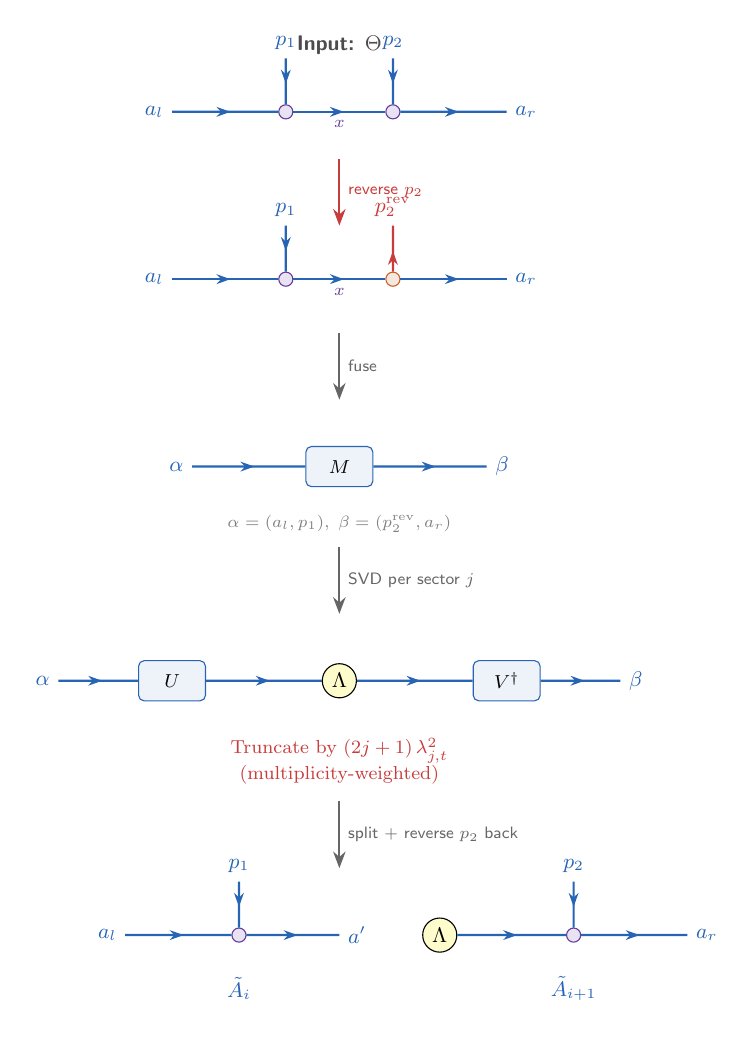
\begin{tikzpicture}[scale=0.85, every node/.style={scale=0.85}]

  % ── Input Theta ──
  \node[font=\small\bfseries\sffamily, text=black!70] at (0,3.5) {Input: $\Theta$};
  \node[fnode] (i1) at (-0.8,2.5) {};
  \node[fnode] (i2) at (0.8,2.5) {};
  \draw[directed, ketcol, thick] (-2.5,2.5) node[left,font=\small]{$a_l$} -- (i1);
  \draw[directed, ketcol, thick] (-0.8,3.3) node[above,font=\small]{$p_1$} -- (i1);
  \draw[directed, ketcol, thick] (i1) -- (i2) node[midway,below,font=\scriptsize,text=fusecol]{$x$};
  \draw[directed, ketcol, thick] (0.8,3.3) node[above,font=\small]{$p_2$} -- (i2);
  \draw[directed, ketcol, thick] (i2) -- (2.5,2.5) node[right,font=\small]{$a_r$};

  % ── Step 1: reverse p2 ──
  \draw[steparrow=revcol, thick] (0,1.8) -- node[right,font=\scriptsize\sffamily,text=revcol]{reverse $p_2$} (0,0.8);

  \node[fnode] (j1) at (-0.8,0) {};
  \node[snode] (j2) at (0.8,0) {};
  \draw[directed, ketcol, thick] (-2.5,0) node[left,font=\small]{$a_l$} -- (j1);
  \draw[directed, ketcol, thick] (-0.8,0.8) node[above,font=\small]{$p_1$} -- (j1);
  \draw[directed, ketcol, thick] (j1) -- (j2) node[midway,below,font=\scriptsize,text=fusecol]{$x$};
  \draw[rdirected, revcol, thick] (0.8,0.8) node[above,font=\small,text=revcol]{$p_2^{\mathrm{rev}}$} -- (j2);
  \draw[directed, ketcol, thick] (j2) -- (2.5,0) node[right,font=\small]{$a_r$};

  % ── Step 2-3: fuse both sides ──
  \draw[steparrow, thick] (0,-0.8) -- node[right,font=\scriptsize\sffamily]{fuse} (0,-1.8);

  \node[stbox=ketcol] (M) at (0,-2.8) {$M$};
  \draw[directed, ketcol, thick] (-2.2,-2.8) node[left,font=\small]{$\alpha$} -- (M.west);
  \draw[directed, ketcol, thick] (M.east) -- (2.2,-2.8) node[right,font=\small]{$\beta$};
  \node[font=\scriptsize, text=black!50, below] at (0,-3.4) {$\alpha=(a_l,p_1),\;\beta=(p_2^{\mathrm{rev}},a_r)$};

  % ── Step 4-5: blockwise SVD ──
  \draw[steparrow, thick] (0,-4.0) -- node[right,font=\scriptsize\sffamily]{SVD per sector $j$} (0,-5.0);

  \node[stbox=ketcol] (U) at (-2.5,-6) {$U$};
  \node[circle, draw=black, fill=yellow!20, inner sep=2pt, font=\small] (L) at (0,-6) {$\Lambda$};
  \node[stbox=ketcol] (V) at (2.5,-6) {$V^\dagger$};
  \draw[directed, ketcol, thick] (-4.2,-6) node[left,font=\small]{$\alpha$} -- (U.west);
  \draw[directed, ketcol, thick] (U.east) -- (L);
  \draw[directed, ketcol, thick] (L) -- (V.west);
  \draw[directed, ketcol, thick] (V.east) -- (4.2,-6) node[right,font=\small]{$\beta$};

  % truncation note
  \node[font=\footnotesize, text=revcol, align=center] at (0,-7.2)
    {Truncate by $(2j+1)\,\lambda_{j,t}^2$\\
     (multiplicity-weighted)};

  % ── Step 6-7: split back ──
  \draw[steparrow, thick] (0,-7.8) -- node[right,font=\scriptsize\sffamily]{split + reverse $p_2$ back} (0,-8.8);

  % Final two tensors
  \node[fnode] (fa) at (-1.5,-9.8) {};
  \draw[directed, ketcol, thick] (-3.2,-9.8) node[left,font=\small]{$a_l$} -- (fa);
  \draw[directed, ketcol, thick] (-1.5,-9.0) node[above,font=\small]{$p_1$} -- (fa);
  \draw[directed, ketcol, thick] (fa) -- (0,-9.8) node[right,font=\small]{$a'$};
  \node[font=\small\bfseries, ketcol] at (-1.5,-10.6) {$\tilde A_i$};

  \node[circle, draw=black, fill=yellow!20, inner sep=2pt, font=\small] (LL) at (1.5,-9.8) {$\Lambda$};

  \node[fnode] (fb) at (3.5,-9.8) {};
  \draw[directed, ketcol, thick] (LL) -- (fb);
  \draw[directed, ketcol, thick] (3.5,-9.0) node[above,font=\small]{$p_2$} -- (fb);
  \draw[directed, ketcol, thick] (fb) -- (5.2,-9.8) node[right,font=\small]{$a_r$};
  \node[font=\small\bfseries, ketcol] at (3.5,-10.6) {$\tilde A_{i+1}$};

\end{tikzpicture}
\end{center}

\begin{costbox}
\textbf{Structural cost:}
One temporary physical-leg reversal on $p_2$.
No $F$-move. No permutation.
\end{costbox}


% ══════════════════════════════════════════════════════════
\section{Summary of Structural Costs}
\label{sec:summary}

\begin{center}
\renewcommand{\arraystretch}{1.3}
\begin{tabular}{l c c c}
\toprule
\textbf{Operation} & \textbf{$\boldsymbol{F}$-moves} & \textbf{$\boldsymbol{R}$-swaps} & \textbf{Reversals} \\
\midrule
Left canonicalization    & 0 & 0 & 0 \\
Right canonicalization   & 0 & 0 & 1 (temporary, physical) \\
Two-site construction    & 0 & 0 & 0 \\
Left environment update  & 2 & $\le 2$ & 0 \\
Right environment update & 2 & $\le 2$ & 0 \\
Effective-$H$ matvec     & 3 & $\le 2$ & 2 (immediate, physical) \\
Two-site SVD split       & 0 & 0 & 1 (temporary, physical) \\
\bottomrule
\end{tabular}
\end{center}

\medskip
\noindent
No operation produces a yoga or monster fusion tree.
All reversals act on boundary physical legs and are sector-wise scalar.
All $F$-moves are local recouplings of adjacent nodes.

% ══════════════════════════════════════════════════════════
\section{Detailed Algebra of the Elementary Moves}
\label{sec:algebra}

For completeness we record the explicit algebraic content of each primitive.

\subsection{$F$-move}

An $F$-move acts on two adjacent fusion nodes sharing an internal edge with
irrep $j_d$, transforming it to a different internal irrep $j_e$:

\begin{center}
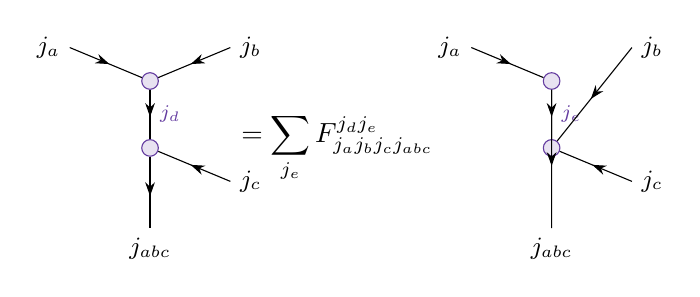
\begin{tikzpicture}[scale=0.85]
  % Left tree
  \node[fnode] (L1) at (0,1) {};
  \node[fnode] (L2) at (0,0) {};
  \draw[directed, black] (-1.2,1.5) node[left,font=\small]{$j_a$} -- (L1);
  \draw[directed, black] (1.2,1.5) node[right,font=\small]{$j_b$} -- (L1);
  \draw[directed, black] (L1) -- (L2) node[midway,right,font=\scriptsize,text=fusecol]{$j_d$};
  \draw[directed, black] (1.2,-0.5) node[right,font=\small]{$j_c$} -- (L2);
  \draw[directed, black] (L2) -- (0,-1.2) node[below,font=\small]{$j_{abc}$};

  % = sum F ...
  \node[font=\normalsize] at (2.8,0) {$= \displaystyle\sum_{j_e} F^{j_d j_e}_{j_a j_b j_c j_{abc}}$};

  % Right tree
  \node[fnode] (R1) at (6,1) {};
  \node[fnode] (R2) at (6,0) {};
  \draw[directed, black] (4.8,1.5) node[left,font=\small]{$j_a$} -- (R1);
  \draw[directed, black] (R1) -- (R2) node[midway,right,font=\scriptsize,text=fusecol]{$j_e$};
  \draw[directed, black] (7.2,1.5) node[right,font=\small]{$j_b$} -- (R2);
  \draw[directed, black] (7.2,-0.5) node[right,font=\small]{$j_c$} -- (R2);
  \draw[directed, black] (R1) -- (6,-1.2) node[below,font=\small]{$j_{abc}$};
\end{tikzpicture}
\end{center}

where the $F$-symbol is related to the Wigner 6-$j$ symbol:
\[
  F^{j_d j_e}_{j_a j_b j_c j_{abc}}
  = (-1)^{j_a + j_b + j_c + j_{abc}} \sqrt{(2j_d+1)(2j_e+1)}
  \begin{Bmatrix} j_a & j_b & j_d \\ j_c & j_{abc} & j_e \end{Bmatrix}.
\]
The degeneracy blocks transform as:
\[
  \boxed{\degblock'_{j_e} = \sum_{j_d} \bigl(F^{-1}\bigr)^{j_d j_e}_{j_a j_b j_c j_{abc}} \;\degblock_{j_d}}
\]

\subsection{$R$-symbol (sibling swap)}

Exchanging the two children of a fusion node with incoming irreps $j_a, j_b$
fusing to $j_c$ costs a phase:
\[
  \boxed{R^{j_c}_{j_a j_b} = (-1)^{j_a + j_b - j_c}}
\]
This is absorbed as a scalar factor into each degeneracy block in the relevant
sector.

\subsection{Index reversal (CUP/CAP)}

Reversing a boundary leg with irrep $j$ transforms each component as:
\[
  \boxed{T'_{j,t,m} = (-1)^{j - m}\,\sqrt{2j+1}\; T_{j,t,-m}}
\]
For a leg that carries only a single irrep sector (such as the spin-$\tfrac{1}{2}$
physical leg), this is a fixed $2\times 2$ matrix applied once.

% ══════════════════════════════════════════════════════════
\section{Design Principles}
\label{sec:principles}

We collect the guiding rules that ensure the strategy works correctly and
efficiently.

\begin{rulebox}[Reversal Rule]
Reverse \textbf{only boundary legs} in hot loops.  If an internal leg needs
reversal, first push it to the boundary via $F$-moves, then reverse, then
swap siblings if needed.
\end{rulebox}

\begin{rulebox}[Permutation Rule]
\textbf{Never} implement a long-range permutation directly.  Instead:
(1)~$F$-move the two target legs to the same node,
(2)~swap siblings,
(3)~absorb the $R$-phase.
\end{rulebox}

\begin{rulebox}[Identity Insertion Rule]
Do not build explicit identity tensors in hot loops.
Conceptually, some basis changes are ``identity insertion + recoupling'',
but in code they should be implemented as: replace the fusion tree template,
apply the inverse $F$-table to the degeneracy blocks.
\end{rulebox}

\begin{rulebox}[Precomputation]
Precompute and cache:
\begin{itemize}[nosep]
  \item Canonical fusion-tree templates for each tensor type
  \item All fixed $F$-move maps (inverse $F$-tables)
  \item All $R$-phase tables for sibling swaps
  \item Reversal factors for physical-leg reversals
  \item Contraction matching tables $E$
  \item Charge-sector routing tables for fusion/splitting
\end{itemize}
Then the runtime kernels reduce to block contractions, small linear
combinations (from $F$), and scalar multiplications (from $R$ and reversals).
\end{rulebox}


% ══════════════════════════════════════════════════════════
\section{Complete Sweep Diagram}
\label{sec:sweep}

The following diagram shows the structural operations during one half-sweep
(left to right) of the two-site finite-vMPS algorithm.

\begin{center}
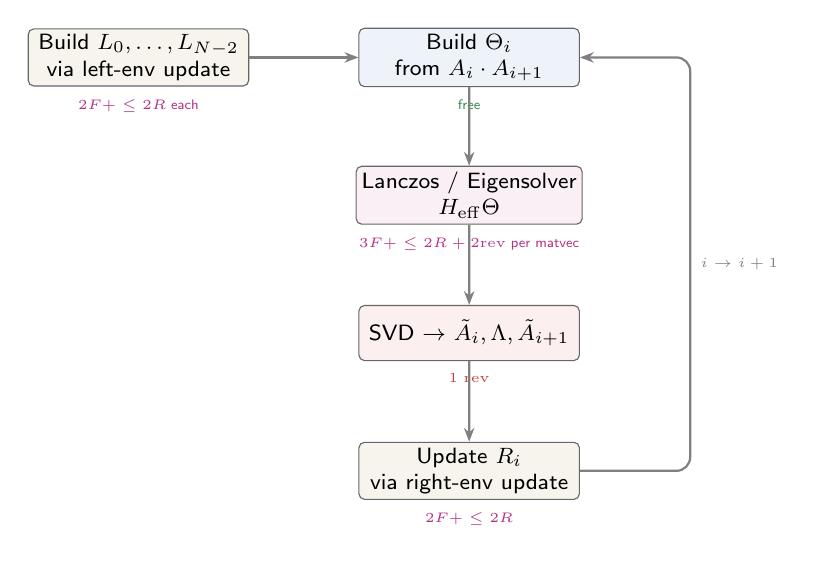
\begin{tikzpicture}[
  scale=0.7,
  box/.style={rectangle, rounded corners=2pt, draw=black!60, fill=#1!8,
              minimum width=28mm, minimum height=7mm, font=\footnotesize\sffamily,
              inner sep=2pt, align=center},
  box/.default={black},
  arr/.style={-{Stealth[length=5pt]}, thick, black!50},
]
  % Column 1: Build environments
  \node[box=envcol] (env) at (0,0) {Build $L_0,\ldots,L_{N-2}$\\via left-env update};
  \node[font=\tiny\sffamily, text=Fcol, below=1pt] at (env.south) {$2F + \le 2R$ each};

  % Column 2: Two-site loop
  \node[box=ketcol] (theta) at (6,0) {Build $\Theta_i$\\from $A_i \cdot A_{i+1}$};
  \node[font=\tiny\sffamily, text=mpocol, below=1pt] at (theta.south) {free};

  \node[box=Fcol] (lanc) at (6,-2.5) {Lanczos / Eigensolver\\$H_{\mathrm{eff}}\Theta$};
  \node[font=\tiny\sffamily, text=Fcol, below=1pt] at (lanc.south) {$3F + \le 2R + 2\mathrm{rev}$ per matvec};

  \node[box=revcol] (svd) at (6,-5) {SVD $\to$ $\tilde A_i,\Lambda,\tilde A_{i+1}$};
  \node[font=\tiny\sffamily, text=revcol, below=1pt] at (svd.south) {$1\;\mathrm{rev}$};

  \node[box=envcol] (rupd) at (6,-7.5) {Update $R_i$\\via right-env update};
  \node[font=\tiny\sffamily, text=Fcol, below=1pt] at (rupd.south) {$2F + \le 2R$};

  % Arrows
  \draw[arr] (env) -- (theta);
  \draw[arr] (theta) -- (lanc);
  \draw[arr] (lanc) -- (svd);
  \draw[arr] (svd) -- (rupd);

  % Loop arrow
  \draw[arr, rounded corners=5pt] (rupd.east) -- ++(2,0) |- node[right,font=\tiny\sffamily,pos=0.25]{$i \to i+1$} (theta.east);

\end{tikzpicture}
\end{center}

% ══════════════════════════════════════════════════════════

\begin{thebibliography}{9}
\bibitem{SSRO2019}
  P.~Schmoll, S.~Singh, M.~Rizzi, and R.~Or\'us,
  ``A programming guide for tensor networks with global $SU(2)$ symmetry,''
  \textit{Ann.\ Phys.}\ \textbf{419}, 168232 (2020);
  \href{https://arxiv.org/abs/1809.08180}{arXiv:1809.08180v2}.
\end{thebibliography}

\end{document}
